\section{Experiment}

\subsection{The purpose of experiment}
There are some questions that we care about. Solving these problems through the controlled experiment we prove that TGCT is meaningful. RQ1: Is the tool-based crowdsourced testing effective in improving the efficiency of crowdsourced testing? RQ2: Does static analysis effectively guide the crowd workers to improve the coverage of crowdsourced testing? 

\subsection{The setup of experiment}
The experiment selected three Android apps: "Jiandou", "QQ Video" and "Music Club". Each application sets up three sets of control experiments during the test: traditional crowdsourced testing, crowdsourced testing that only includes automated test guidance, and crowdsourced testing guided by automated testing and static analysis(TGCT). We define $\left|C\right|$ as the traditional crowdsourced testing process, $\left|A\right|$ as only partially guided crowdsourced testing, $\left|T\right|$ as the TGCT mechanism.

\subsection{The result of experiment}
In order to answer RQ1, we define the efficiency of the crowdsourced test as the number of exceptions triggered per unit time. In the experiment $\left|C\right|$ and $\left|T\right|$, the number of non-repeating exceptions that the crowd workers discovered had been counted every minute. We got three line charts of the number of exceptions in three applications over time, as shown in Figure\ref{fig:xi}.
\begin{figure}[htbp]
\centering
\subfigure["Jiandou".]{
\begin{minipage}[t]{0.33\linewidth}
\centering
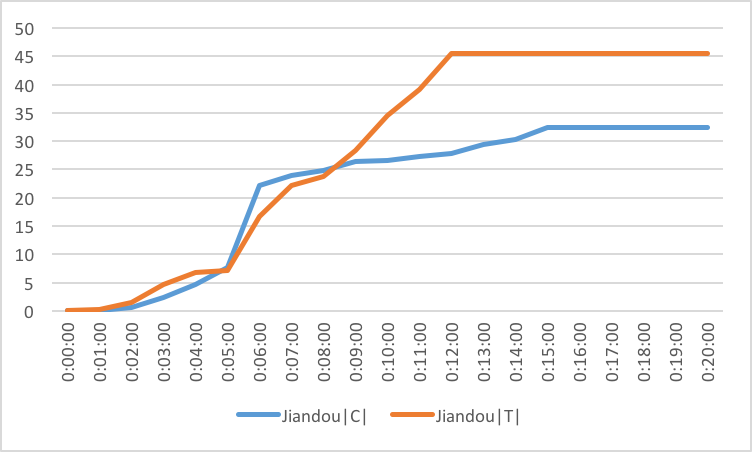
\includegraphics[width=1in]{fig/8-1.png}
%\caption{fig1}
\end{minipage}%
}%
\subfigure["QQ Video".]{
\begin{minipage}[t]{0.33\linewidth}
\centering
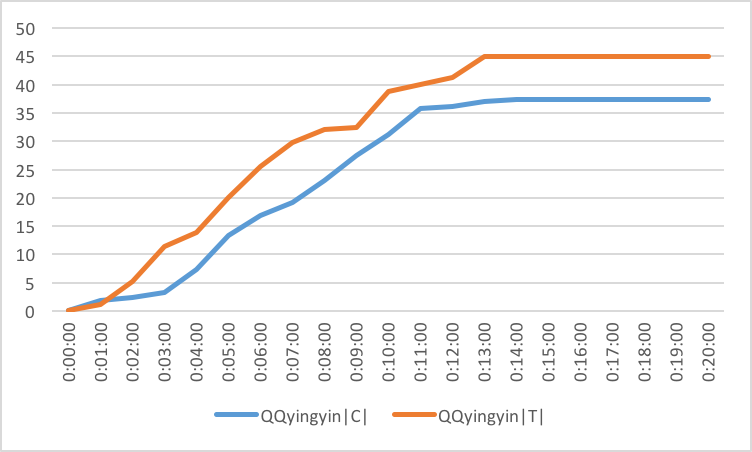
\includegraphics[width=1in]{fig/8-3.png}
%\caption{fig2}
\end{minipage}%
}%
\subfigure["Music Club".]{
\begin{minipage}[t]{0.33\linewidth}
\centering
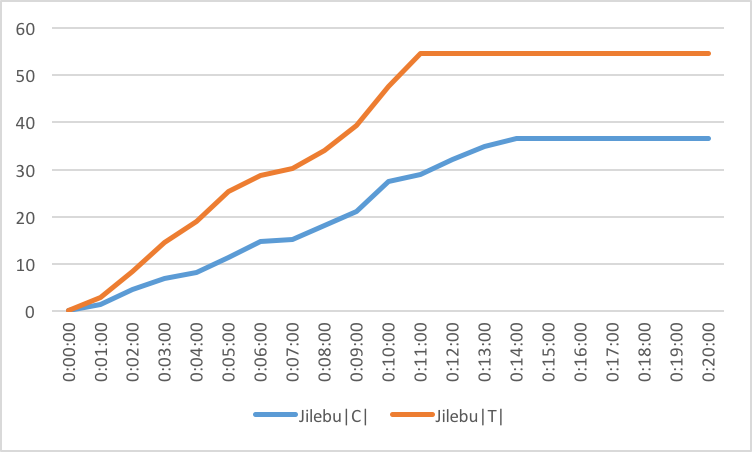
\includegraphics[width=1in]{fig/8-2.png}
%\caption{fig2}
\end{minipage}
}%
\centering
\caption{Line chart of the number of exceptions in three applications over time.}
\label{fig:xi}
\end{figure}

From the overall trend of the three figures, tool-guided crowd workers trigger exceptions faster and more.

In order to answer RQ2, we count the proportion of windows that are not covered by these three applications. As shown in Table\ref{fig:xixi}, we showed the coverage of the uncovered window of the "Jiandou" app.
\begin{table}[tb]
\caption{The Coverage in "jiandou".}
\begin{center}
\begin{tabular}{|c|c|c|} %l(left)居左显示 r(right)居右显示 c居中显示
\hline 
Element&$\left|A\right|$ Coverage&$\left|T\right|$ Coverage\\
\hline  
BookDetailsActivity&5.4 / 12&5 / 12\\
\hline 
ActorDetailsActivity&5.8 / 12&6 / 12\\
\hline 
AlertDialog&0.2 / 6&4 / 6\\
\hline 
TOTAL&10.2 / 30&15 / 30\\
\hline 
\end{tabular}
\label{fig:xixi}
\end{center}
\end{table}

Then we compare the result of experiment $\left|T\right|$ with the experiment $\left|A\right|$ to verify the effectiveness of the guide mechanism for uncovered window transition according to the average code coverage of the starting window.
According to the calculation results of all the code coverage of the uncovered window, we found that for crowd workers, the guidance of static source analysis can effectively improve the coverage of crowdsourced testing.